% -*-coding: utf-8 -*-
\documentclass[11pt,a4paper]{report}

\newif\ifrelease % new boolean variable release. True = include some fancy content
\releasefalse % and set it

\usepackage[czech]{babel}
\usepackage[utf8]{inputenc}
\usepackage[IL2]{fontenc}

\usepackage{amsmath}
\usepackage{amsthm}
\usepackage{amstext}
\usepackage{amsfonts}
\usepackage{epsfig}
\usepackage{graphicx}
\usepackage{color}
\usepackage{multirow}
\usepackage{booktabs}
\usepackage[abs]{overpic}
\setlength\unitlength{1mm}
\usepackage{fancyvrb}

%\usepackage[justification=centering]{caption}
\ifrelease
	\usepackage{pdfpages}
\fi
\usepackage[pagebackref=true]{hyperref} % tento balicek by mel byt na konci baliku!

\hypersetup{
	pdfauthor={Ladislav Horký},
	pdftitle={Použití fuzzy logiky ve zpracování obrazu na GPU}
}

%% Nastavení zrcadla sazby
\usepackage{calc}
\setlength{\textheight}{9in}
\setlength{\textwidth}{6in}
\setlength\oddsidemargin{(\paperwidth-\textwidth)/2 - 1in}
\setlength\evensidemargin{(\paperwidth-\textwidth)/2 - 1in}
\setlength\topmargin{(\paperheight-\textheight-\headheight-\headsep-\footskip)/2 - 1in}

%\parindent=0pt % odsazení 1. řádku odstavce
%\parskip=4pt   % mezera mezi odstavci

\ifrelease
	\hypersetup{pdfborder={0 0 0}} % no borders around links
\else
	\hypersetup{colorlinks=true} % colour links instead of borders
\fi
% =========================================================
% Ams definice

\theoremstyle{plain}
\newtheorem{define}{Definice}
\newtheorem{theo}{Věta}


% Vlastní příkazy:==========================================
\newif\ifshownotes % zobraz poznámky level 1
\shownotestrue
\newif\ifshownotesadd % zobraz poznámky level 2
\shownotesaddtrue

\newcommand{\LAs}{\L A_{sqrt}}
\newcommand{\rl}{\textup{(}}
\newcommand{\rr}{\textup{)\,}}
\ifshownotes
    \newcommand{\note}[1]{{\color{green}{\emph{#1}}}}
\else
    \newcommand{\note}[1]{}
\fi
\ifshownotesadd
    \newcommand{\notea}[1]{{\color{green}{\emph{#1}}}}
\else
    \newcommand{\notea}[1]{}
\fi
\newcommand{\LL}{\mathbf{L}}
\newcommand{\sqr}{\mathrm{sqrt}}
\newcommand{\LAsq}{$\mathrm{\L A_{sqrt}}$ }
\newcommand{\beq}{\begin{equation}}
\newcommand{\eeq}{\end{equation}}
\newcommand{\xx}{\mathbf{x}}
\newcommand{\yy}{\mathbf{y}}
\newcommand{\f}{\mathrm{f}}
\newcommand{\g}{\mathrm{g}}
\newcommand{\PP}{\mathcal{P}}
\newcommand{\QQ}{\mathcal{Q}}
\newcommand{\NN}{\mathcal{N}_{R}(x_{i,j,k})}
\newcommand{\MM}{\mathcal{M}_R}
\newcommand{\Lw}{{\mathrm{L^w}_{i,j,k}}}
\newcommand{\Nb}{{\mathrm{N}_{i,j,k}}}
\newcommand{\WL}{{\mathrm{WL}_{i,j,k}}}
\newcommand{\EE}{\mathrm{E}}
\newcommand{\DD}{\mathrm{D}}
\newcommand{\OO}{\mathrm{O}}
\newcommand{\CC}{\mathrm{C}}
\newcommand{\MED}{\mathrm{MED}}
\newcommand{\BES}{\mathrm{BES}}
\newcommand{\kk}{\textit{k}}
\newcommand{\ccc}{\textit{c}}
\newcommand{\et}{\;\,\mathrm{et}\;\,}
\newcommand{\Cpp}{C\raisebox{0.15ex}[0ex][0ex]{++}}

\newcommand{\Nn}{\mathbb{N}}
\newcommand{\RR}{\mathbb{R}}
\newcommand{\Imageman}{{\tt ImageManager<imDataType>}}
\newcommand{\Imageinfo}{{\tt ImageInfo}}
\newcommand{\imDataType}{{\tt imDataType}}
\newcommand{\Analyze}{Analyze$^{\mathrm{\textsc{tm}}}$ 7.5}
\newcommand{\image}{{\tt image}}
\newcommand{\imageGpu}{{\tt imageGpu}}
\newcommand{\bl}[1]{\textcolor[rgb]{0,0,1}{#1}} % prostě fancyverbatim neumí textbf
\newcommand{\cy}[1]{\textcolor[rgb]{1,0,1}{#1}}
\newcommand{\FERMI}{FERMI$^{\mathrm{\textsc{tm}}}$}
\newcommand{\Vr}{\Verb[commandchars = \\\{\}]}


% Definice makra pro české uvozovky:
\def\bq{\mbox{\kern.1ex\protect\raisebox{-1.3ex}[0pt][0pt]{''}\kern-.1ex}}
\def\eq{\mbox{\kern-.1ex``\kern.1ex}}
\def\ifundefined#1{\expandafter\ifx\csname#1\endcsname\relax }%
\ifundefined{uv}%
        \gdef\uv#1{\bq #1\eq}
\fi

% Dělení slov:=============================================
\hyphenation{pře-klá-da-jí-cí}

% =========================================================
\begin{document}

\ifrelease
	% -*-coding: utf-8 -*-
\newcommand{\cvut}{České Vysoké Učení Technické v~Praze}
\newcommand{\fjfi}{Fakulta Jaderná a Fyzikálně Inženýrská}
\newcommand{\km}{Katedra matematiky}
\newcommand{\obor}{Inženýrská Informatika}
\newcommand{\zamereni}{Softwarové Inženýrství a Matematická Informatika}

\newcommand{\nazevcz}{Paralelní implementace fuzzy filtrů ve zpracování obrazu na GPU}
\newcommand{\nazeven}{Parallel Implementation of Fuzzy Filters in Image Processing on GPU}
\newcommand{\autor}{Ladislav Horký}
\newcommand{\rok}{2011}
\newcommand{\vedouci}{Ing. Tomáš Oberhuber Ph.D.}

\newcommand{\pracovisteVed}{Katedra matematiky \\
    České Vysoké Učení Technické v~Praze}
\newcommand{\konzultant}{doc. Ing. Jaromír Kukal Ph.D.}
\newcommand{\pracovisteKonz}{Katedra softwarového inženýrství \\
    České Vysoké Učení Technické v~Praze}

\newcommand{\klicova}{Fuzzy logika, zpracování obrazu, robustní filtry, GPGPU, CUDA}
\newcommand{\keyword}{Fuzzy Logic, image processing, robust filters, GPGPU, CUDA}
\newcommand{\abstrCZ}{

    Cílem práce bylo zjistit možnosti urychlení filtrace 3D medicínských dat na GPU u obrazových filtrů postavených na fuzzy logice. Nejprve bylo provedeno zobecnění použité teorie do 3D a následná implementace na CPU v jazyce \Cpp ~při použití nejlepších dostupných algoritmů. Implementace na GPU byla provedena v prostředí NVIDIA CUDA C a použité algoritmy a optimalizace jsou až na jeden původní. Hodnoty urychlení jsou na celé škále 2,3krát až 60krát (kde jsme naráželi na pro hardware nevhodné rozměry zpracovávaných dat) a u jednodušších filtrů tak došlo ke zkrácení doby výpočtu na testovacích datech na jednotky ms. Navíc byla provedena teoretická diskuse schopnosti filtrů medián, BES, H.-L. medián a WBES odstraňovat kontaminovaný gaussovský šum i s praktickými příklady.}
\newcommand{\abstrEN}{

    The aim of the thesis was to determine the possibility of speeding up 3D medical image processing on GPU using filters based on Fuzzy logic. First, generalization of the theory into 3D and subsequent implementation on CPU using \Cpp ~language and the best possible algorithms was carried out. Implementation on GPU was made within the NVIDIA CUDA C enviroment with all but one used algoritms and optimizations being original. The gained speedup ranges from nearly 60 times down to 2,3 times (where most difficulties with input data dimensions occured) and the total duration of computation dropped for some filters below 10 ms. As a bonus, a theoretical discussion on median, BES, H.-L. median and WBES capability of suppressing contaminated gaussian noise together with practical expamples were carried out.}

%%% zde zacina kresleni dokumentu

% titulní strana
\thispagestyle{empty}

\begin{center}
	{\Large  \bf  \cvut\\[2mm] \fjfi }
	\vspace{10mm}

	\begin{tabular}{c}
	{\bf \km}\\
	{\bf Obor: \obor}\\
	{\bf Zaměření: \zamereni}
	\end{tabular}

	\vspace{10mm} \epsfysize=20mm  \epsffile{cvut-logo-bw-600} \vspace{15mm}

	{\LARGE
	\textbf{\nazevcz}
	\par}

	\vspace{5mm}

	{\LARGE
	\textbf{\nazeven}
	\par}

	\vspace{30mm}
	{\Large BAKALÁŘSKÁ PRÁCE}

\end{center}

\vfill
{\large
\begin{tabular}{rl}
Vypracoval: & \autor\\
Vedoucí práce: & \vedouci\\
Rok: & \rok
\end{tabular}
}

% zadání bakalářské práve
\newpage
\thispagestyle{empty} Před svázáním místo téhle strany \fbox{vložíte zedání práce} s podpisem
děkana (bude to jediný oboustranný list ve Vaší práci) !!!!

% prohlášení
\newpage
\thispagestyle{empty}
~
\vfill


{\bf Prohlášení}

\vspace{0.5cm}
Prohlašuji, že jsem svou bakalářskou práci vypracoval samostatně a použil jsem pouze podklady
(literaturu, projekty, SW atd.) uvedené v přiloženém seznamu.

\vspace{5mm}V Praze dne ....................\hfill
    \begin{tabular}{c}
    ........................................\\
    \autor
    \end{tabular}

% poděkování
\newpage
\thispagestyle{empty}
~
\vfill

{\bf Poděkování}

\vspace{5mm}
Rád bych poděkoval panu Ing. Tomáši Oberhuberovi Ph.D. a panu doc. Ing. Jaromíru Kukalovi Ph.D. za podporu, velkou vstřícnost a cené rady a zkušenosti, které mi při vedení práce a konzultacích v bohaté míře poskytovali.

\begin{flushright}
\autor
\end{flushright}

% strana s abstraktem
\newpage
\thispagestyle{empty}

\newbox\odstavecbox
\newlength\vyskaodstavce
\newcommand\odstavec[2]{%
    \setbox\odstavecbox=\hbox{%
         \parbox[t]{#1}{#2\vrule width 0pt depth 4pt}}%
    \global\vyskaodstavce=\dp\odstavecbox
    \box\odstavecbox}
\newcommand{\delka}{120mm}

\hspace{-0.9cm}
\begin{tabular}{ll}
  {\em Název práce:} & ~ \\
  \multicolumn{2}{l}{\odstavec{\textwidth}{\bf \nazevcz}} \\[5mm]
  {\em Autor:} & \autor \\[5mm]
  {\em Obor:} & \obor \\
  {\em Druh práce:} & Bakalářská práce \\[5mm]
  {\em Vedoucí práce:} & \odstavec{\delka}{\vedouci \\ \pracovisteVed} \\[5mm]
  {\em Konzultant:} & \odstavec{\delka}{\konzultant \\ \pracovisteKonz} \\[5mm]
  \multicolumn{2}{l}{\odstavec{\textwidth}{{\em Abstrakt:} ~ \abstrCZ \\ }} \\[5mm]
  {\em Klíčová slova:} & \odstavec{\delka}{\klicova} \\[20mm]

  {\em Title:} & ~\\
  \multicolumn{2}{l}{\odstavec{\textwidth}{\bf \nazeven}}\\[5mm]
  {\em Author:} & \autor \\[5mm]
  \multicolumn{2}{l}{\odstavec{\textwidth}{{\em Abstract:} ~ \abstrEN \\ }} \\[5mm]
  {\em Key words:} & \odstavec{\delka}{\keyword}
\end{tabular}
 % úvodní strany
\fi

    \tableofcontents

    \addcontentsline{toc}{chapter}{Úvod}
    \chapter*{Úvod}
        % -*-coding: utf-8 -*-

% cíl, trend

% aplikace zpracovává 3D obraz

Práce je zaměřená na urychlení známých obrazových filtrů na GPU. Přesouvání výpočtů na GPU má dnes už ve vědecké komunitě své pevné místo a k řadě problémů, jako např. třídění polí a konvoluce v obraze, jsou již k dispozici knihovny GPU využívající. Náš problém se však menšími rozměry vstupních dat -- je třeba třídit pole pouze o stovkách prvků -- tomuto mainstreamu poněkud vymyká. Algoritmy, které urychlí fitraci na dobu milisekund až desítky milisekund mohou být výhledově použity v aplikacích, které potřebují výsledky filtrů v reálném čase. To může být naříklad program s okamžitou vizuální zpětnou vazbou, umožňující laikovi sestavit si potřebný filtr pomocí jednoduchého skládání filtrů a manipulací s jejich parametry.

Jako teoretický základ filtrů byla použita fuzzy logika, konkrétně \L ukasiewiczova algebra s odmocninou, která je přímo aplikovatelná na data tak, jak jsou v počítači reprezentována a je vhodná pro konstrukci sítí filtrů, při jíž se může urychlení na GPU taktéž bohatě uplatnit.
Popis je zaměřen na typové filtry ze tříd morfologický a statisticky motivovaných filtrů, které jsou posléze i implementovány.

V práci nebudeme porovnávat urychlení konkrétních algoritmů mezi CPU a GPU, ale urychlení celých filtrů. Při implementaci jsou tak na CPU a GPU použity pro ten samý filtr vždy rozdílné algoritmy, z nichž každý je optimalizován na rychlost a konkrétní platformu -- díky hardwarovým omezením na GPU klademe na kód jiné požadavky.

Implementace na CPU je provedena v jazyce \Cpp ~za použítí nejlepších dostupných algoritmů, na GPU je použito prostředí NVIDIA CUDA C a použité algoritmy a optimaliazce jsou až na výjimky původní.

Za svůj autorský podíl na práci považuji sjednocení symboliky v rešeršní části práce a diskusi citlivosti filtrů na kontaminovaný gaussovský šum. Dále pak návrh a realizaci programu pro testování urychlení filtrů na GPU v prostředí CUDA C a diskusi problematiky třídění malých polí na GPU.


    \chapter{Fuzzy logika}
        % Lukasiewiczova algebra s odmocniou
            % Konstrukce matematického modelu
                % Svaz
                % Lukasiewiczova algebra
                % Lukasiewiczova algebra s odmocninou
            % Fuzzy-logická funkce
            % Používané operátory
        % Citlivost
            % Přesnost celočíselné aritmetiky
        % Reprezentace obrazových dat
            % Maska
        % Filtry
            % Typologie filtrů
                % Morfologické
                % Statistické
            % Citlivost filtrů
            % Porovnání s lineárními filtry

        %% -*-coding: utf-8 -*-

    \chapter{Implementace na CPU}\label{cpu impl}
        % Celočíselná aritmetika
            % Přesnost
        % Práce s 3D obrazovými daty
            % Načítání, ukládání (lehce k .hdr, .img)
            % Uchování dat v paměti (řešení okrajů...)
        % Masky, strukturní elementy
        % Implementace filtrů
            % Quickselect

         % -*-coding: utf-8 -*-

        % Celočíselná aritmetika
            % Přesnost
        % Práce s 3D obrazovými daty
            % Načítání, ukládání (lehce k .hdr, .img)
            % Uchování dat v paměti (řešení okrajů...)
        % Masky, strukturní elementy
        % Implementace filtrů
            % Quickselect
%=========================================================================

V této kapitole popíšeme implementaci filtrů a nejdůležitějších podpůrných struktur na CPU v \Cpp. Před samotným popisem kódu ještě prodiskutujeme téma přesnosti výpočtů.

    \section{Celočíselná aritmetika}

    Při implementaci jsme se omezili pouze na dva celočíselné typy {\tt unsigned char} (0-255) a {\tt unsigned short} (0-65535). Jednak proto, že vstupní data jsou často právě v rozsahu 0-255 a zadruhé, lidské oko stejně není schopné objektivně rozeznat spojitější škálu -- zvláště u jednokanálových (odstíny šedi) obrazů. Neceločíselné typy jsme úplně vynechali ze stejného důvodu, počítání s nimi je navíc podstatně pomalejší. Výběr konkrétního datového typu lze v kódu jednoduše provést pomocí parametru šablony.

        \subsection{Přesnost}

        Jedinou operací, která vnáší do výpočtů chybu, je celočíselné dělení\footnote{ostatní operace ovšem přenášejí chyby již vzniklé} -- násobení, sčítání a odčítání jsou přesné a jiné operace nepoužíváme. Díky požadavkům na teorii (uzavřenost vůči operacím) nikdy nebude docházet k chybám z ořezání výsledku do rozsahu datového typu, nebo jeho přetečení, a můžeme tak analyzovat pouze zaokrouhlovací chyby:

        Hrubý odhad chyby dělení nám dává následující nerovnost:
        \beq
        \frac{m}{n} \le \Big\lfloor \frac{m}{n} \Big\rfloor +1 \qquad m \in \Nn_0, \, n \in \Nn
        \eeq
        Abychom chybu zbytečně nezveličovali, budeme dále uvažovat $\delta \in \RR^+$ a přesnější odhad:
        \beq
        \frac{m}{n} = \Big\lfloor \frac{m}{n} \Big\rfloor + \Big\{ \frac{m}{n} \Big\} = \Big\lfloor \frac{m}{n} \Big\rfloor + \delta
        \eeq
        Jednoduchou úvahou dospějeme k závěru, že největší možná desetinná část při dělení $n$ je $\frac{n-1}{n}$, a tedy:
        \beq
        \delta \leq \frac{n-1}{n}
        \eeq

        Chyba dělění je navíc vždy kladná, a násobení a sčítání jí kladnou nechá. Pokud nepoužijeme ve výpočtech rozdíl, který znaménko chyby samozřejmě nezachová, můžeme toho v odhadech využít. Aritmetiku chyby (obecně se znaménkem) shrnuje tabulka~\ref{tabulka max chyby}. Všechny operace v \LAsq můžeme redukovat na operace uvedené v tabulce (viz výše).

        \begin{table}[h]\label{tabulka max chyby}
    \begin{center}
    \begin{tabular}{lll}
      \toprule
      Operace & Popis & Chyba\\
      \midrule
      $\frac{m\pm\delta_1}{n} \; n \neq 0 $ & Celočíselné dělení konstantou & $\pm \Big( \frac{\delta_1}{n} + \frac{n-1}{n}\Big)$ \\
      $(m\pm\delta_1)+(n\pm\delta_2) $      & Sčítání                       & $\pm \,(\delta_1+\delta_2)$ \\
      $(m\pm\delta_1)-(n\pm\delta_2) $      & Odčítání                      & $\pm \,(\delta_1+\delta_2)$ \\
      $n(m\pm\delta_1) $                    & Násobení konstantou           & $\pm \,n\delta_1$ \\
      $\max(m\pm\delta_1,n\pm\delta_2) $    & Maximum                       & $\pm \max(\delta_1,\delta_2)$ \\
      $\min(m\pm\delta_1,n\pm\delta_2) $    & Minimum                       & $\pm \max(\delta_1,\delta_2)$ \\
      \bottomrule
    \end{tabular}
    \caption{Chyba celočíselných aritmetických operací, $m,n \in \Nn_0, \,\delta_1,\delta_2 \in \RR^+$}
    \end{center}
        \end{table}

        Jako příklad uveďme chybu WBES: na vstupu je použit Walshův list (dělení dvěmi, chyba $0.5$), poté sčítání a dělení čtyřmi. Nepoužíváme rozdíl, takže celočíselný výsledek bude menší nebo rovnen skutečnému:
        \beq
        \delta = +\Big( \frac{0.5+0.5+0.5+0.5}{4} + \frac{4-1}{4} \Big) = +1.25
        \eeq
        Pokud Walshův list uložíme do většího datového typu a průměrování provedeme až na konci (jedinné dělení osmi), můžeme chybu stlačit až na $+0.875$. Dělení (pouze to vnáší chybu) se pomocí rozšíření datového typu obecně snažíme přesouvat až nakonec výpočtu, abychom počítali co nejdéle přesně a minimalizovali tak chybu. Závěrem dodejme, že chyby v příkladu jsou absolutní -- při použití {\tt unsigned char} bude relativní chyba $\frac{+1.25}{256}$, při použití {\tt unsigned short} bude ještě 256krát menší. \notea{ chyba je malá, opakovaným filtrování by došlo k degradaci dat dříve díky rozmazání filtrem, než chybou -- vyzkoušet v příkladě (př 100x WBES char, neoptimalizovaný VS 100 WBES short optimalizovaný)}

    \section{Práce s 3D obrazovými daty}

    O uchovávání, načítání a ukládání 3D dat se v kódu stará šablonová třída \Imageman, geometrii obrazu má na starost abstaktní třída \Imageinfo. Celkový přehled struktury kódu pracujícíh s 3D obrazem lze najít s podrobnějším popisem v příloze~\ref{struktura kódu}. Nyní nám stačí vědět, že 3D obraz je opatřen nulovými okraji (viz sekce~\ref{lokální zprac}) a v paměti uložen jako lineární pole.

    \section{Maska, strukturní element}

    Správu strukturních elementů má na starosti třída {\tt SEManager}, samotné strukturní elementy jsou uloženy ve struktuře {\tt structEl}, kterou pro přehlednost uvádíme zde:

    \begin{Verbatim}[commandchars = \\\{\}]
\bl{typedef struct} _structEl \{
    \bl{string} name;       // název pro pozdější vyhledání
    \bl{int} *wList;        // Lw z teorie, pole o délce = capacity
    \bl{unsigned} capacity; // kapacita masky
    \bl{unsigned} *mask;    // váhy okolních voxelů, neparsovaný vstup, viz dále
\} structEl;
    \end{Verbatim}

    \subsection{Formát}

    Všechny strutury se snažíme optimalizovat na rychlost. Při filtraci budeme chtít rychle a elegantně přistupovat k okolí zpracovávaného voxelu, nejlépe takto (za předpokladu, že {\tt src} ukazuje na zpracovávaný obrázek a {\tt SE} je strukturní element):

    \begin{Verbatim}
iTyVoxelOkoli = src[indexZpracVoxelu + SE.wList[i]]; // 0<= i<SE.capacity
    \end{Verbatim}

    Atribut {\tt wList} bude tedy obsahovat rozdíly indexů centrálního voxelu a okolních voxelů. Masku chceme zadávat v co možná nejjednodušším formátu, jako vhodně uspořádané jednorozměrné pole (přílkad maska $3\times 3\times3$ -- poloměr $R = 1$):

    \begin{Verbatim}[commandchars = \\\{\}]
\bl{unsigned} maska[] = \{
    0,1,0,  1,1,1,  0,1,0,
    1,1,1,  1,4,1,  1,1,1,
    0,1,0,  1,1,1,  0,1,0
\};
    \end{Verbatim}

    Na masku se při zápisu díváme shora a zapisujeme jednotlivé vrstvy, jak je vidíme: nejlevější blok je horní vrstva, nejpravější spodní. Výhodou tohoto formátu je, že pokud bychom chtěli načítat masku ze souboru (neimplementováno), můžeme ji zapsat zcela stejně, protože při klasickém načítání po řádcích se formát nepoškodí. Maska s poloměrem $R = 2$ bude mít analogicky $5$ bloků $5\times 5$.

    Popis načítání masek a další práce s nimi je v příloze~\ref{struktura kódu}.

    \section{Implementace filtrů}

    Filtry jsou obsaženy v abstraktní šablonové třídě {\tt Filter}, což je vlastně pouze kontejner na funkce s několika podpůrnými statickými proměnnými. Před voláním jakékoliv funkce je nutno tyto inicializovat pomocí {\tt Init(sem)}, které se předá ukazatel na {\tt SEManager} (musí již být konkretizovaný). Inicializace dále dopočítá geometrické konstanty použité při procházení datového pole na CPU. Popis formátu filtrů je opět v příloze~\ref{struktura kódu}.

    \subsection{Implementace a optimalizace na CPU}

        Nyní probereme postupně implementační a optimalizační záležitosti vztahující se na veškerý kód na CPU a posléze implementaci jednotlivých filtrů.

        \paragraph{Obecně} se snažíme optimalizovat na rychlost. Vyhýbáme se častým alokacím a dealokacím proměnných v cyklech a opakovaně volaných funkcích, k čemuž \Cpp možností definovat proměnnou kdekoliv celkem svádí -- překladač sice dost těchto případů optimalizuje sám, ale není od věci mu naznačit, že pamětí může plýtvat. \note{prakticky vyzkoušet?}. Taktéž se při větvení programu vyplatí tvořit stromy podmínek spíše do hloubky, než do šířky -- snížíme průměrný počet podmínek, kterými je třeba projít. Toto se samozřejmě týká časově náročných částí kódu, v těch časově nepodstatných je naopak lepší upřednostnit přehlednost. \note{není to už moc obecné?}

        \paragraph{Sekvenční zpracování 3D dat} zajišťuje pro všechny filtry parametrické makro {\tt BEGINFOR3D(pos)} a {\tt ENDFOR3D}, díky kterému projde parametr {\tt pos} pouze ty správné indexy z pole dat. Z celého pole 3D dat totiž musíme zpracovat pouze obraz, nikoliv okraje. Makro obsahuje tři for-cykly a počítá index {\tt pos}, přičemž minimalizuje počet operací k tomu potřebných. Použití ({\tt src} je opět zdroj):

        \begin{Verbatim}[commandchars = \\\{\}]
\bl{unsigned long} idx;
BEGINFOR3D(idx)
    // tělo filtru
    // zpracovávaný voxel je src[idx]
ENDFOR3D
        \end{Verbatim}

        \paragraph{Morfologické filtry} eroze a dilatace jsou implementovány zcela v souladu s definicí v \ref{Filtry}. Pouze detektor hran je lehce optimalizován -- operaci $\DD(\PP) \ominus \EE(\PP)$ můžeme samozřejmě přesunout na úroveň voxelů:

        \begin{Verbatim}[commandchars = \\\{\}]
\bl{unsigned long} idx;
\bl{unsigned} i;
\bl{imDataType} min,max;
BEGINFOR3D(idx)
    min = max = src[idx + SE.wList[0]];
    \bl{for}(i=1; i<SE.capacity; i++)\{
        \bl{if}(min > src[idx + SE.wList[i]]) min = src[idx + SE.wList[i]];
        \bl{if}(max < src[idx + SE.wList[i]]) max = src[idx + SE.wList[i]];
    \}
    dst[idx] = max - min;
ENDFOR3D
        \end{Verbatim}

        Zmíněné tři filtry jsou implementačně triviální, zajímavé ale bude jejich urychlení na GPU, kde se vzhledem k jednoduchosti operací dostaneme na hranici hardwarových možností.

        \paragraph{Statisticky motivované filtry} jsou implementačně nejzajímavější, neboť je při nich třeba z pole hodnot vybrat obecně několikrát \kk-tý prvek. Implementovány jsou čtyři základní filtry: {\tt Median}, {\tt WMedian}, {\tt BES} a {\tt WBES}. Jejich jádrem na CPU jsou dvě funkce {\tt MedianFindOpt} a {\tt UniBESFind}, které operují buď nad polem vytvořeným z obrazových dat podle {\tt wList}, nebo nad příslušným Walshovým seznamem\footnote{seznam je zde pouze součást názvu, samozřejmě je implementován jako pole} vytvořeným z tohoto pole.

        Funkce {\tt MedianFindOpt(base,length)} částečně setřídí pole {\tt base} o délce {\tt length} tak, že se na indexu {\tt length/2} bude nacházet medián (případně na indexech {\tt (length/2)} a {\tt (length/2)-1} prvky potřebné ke konstrukci mediánu pro {\tt length} sudé).

        \begin{Verbatim}[commandchars = \\\{\}]
\bl{bool} MedianFindOpt(\bl{imDataType} *base, \bl{unsigned} initBaseLength)\{
    \bl{static int} first, last;
    \bl{static unsigned} length = 0, rising, falling, pivot, itemsToFind, upper, lower;
    \bl{static imDataType} swap;
    \bl{if}(initBaseLength != 0)\{      //inicializace
        length = initBaseLength;
        upper = length/2;
        lower = length/2-1+length\%2;  //lichá délka bude stejný jako upper
        \bl{return true};
    \}
    itemsToFind = 2-initBaseLength\%2; //2 nebo 1 prvek
    first = 0;	
    last = length-1;

    \bl{while}(1)\{                 //vnější smyčka
        \bl{if}(!progress) \bl{return true};
        \bl{if}(last-first < EFFICIENT_MAX)\{
            \bl{if}(last-upper < lower - first)
                InsertSortMax(base,first,last,last-lower+1);	
            \bl{else}
                InsertSortMin(base,first,last,upper-first+1);	
            \bl{return true};
        \}
        pivot = first;
        rising = first+1;
        falling = last;
        \bl{if}(base[rising] > base[falling]) SWAP(rising,falling);
        \bl{if}(base[rising] > base[pivot]) SWAP(rising,pivot);
        \bl{if}(base[falling] < base[pivot]) SWAP(falling,pivot);

        \bl{while}(1)\{			     //vnitřní smyčka				
            \bl{do} falling--; \bl{while}(base[falling] > base[pivot]);
            \bl{do} rising++; \bl{while}(base[rising] < base[pivot]);
            \bl{if}(rising > falling)\{	
                SWAP(pivot,falling);
                \bl{break};
            \}\bl{else}\{					
                SWAP(rising,falling);
            \}
        \}
        \bl{if}(falling > upper) last = falling-1;	
        \bl{else if}(falling < lower) first = falling+1;
        \bl{else}\{
            progress--;
            \bl{if}(falling == lower) first = falling+1;
            \bl{else} last = falling-1;
        \}
    \}
\}
        \end{Verbatim}

        Funkce je volána při zpracování každého voxelu, proto jsou proměnné alokovány staticky, tudíž se nedealokují po opuštění funkce a šetří čas při správě paměti. K nalezení požadovaných prvků je použit algoritmus \emph{Quickselect} založený a \emph{Quicksort}u, který je i s optimalizacemi popsán v \cite{Numerical Recipes}. V základní verzi algoritmus pracuje následovně:
        \begin{enumerate}
          \item V poli vybereme pivota (obyčejně nejlevější prvek) {\tt p}
          \item Zbytek pole procházíme ukazatelem zleva, dokud nenajdeme prvek $\ge$ {\tt p}
          \item Stejně procházíme zprava, dokud nenajdeme prvek $\le$ {\tt p}
          \item Tyto dva prvky prohodíme
          \item Pokračujeme dokud se ukazatele nepřekříží, na toto místo vložíme {\tt p}
          \item Stejný postup aplikujeme na levé, nebo pravé podpole (pivot je již na svém místě), podle toho, jesti pivot skončil pod, nebo nad mediánem (obecně \kk-tým prvkem)
        \end{enumerate}

        Časově nejnáročnější je vnitřní smyčka algoritmu, tu můžeme urychlit odebráním kontrol, zda jsme s ukazatelem nevyjeli mimo pole, což se může stát, pokud by byl pivot nejmenším, nebo největším prvkem v prohledávaném úseku. To vyřešíme tak, že pivota zvolíme jako medián tří prvků, z nichž největší umístíme nakonec prohledávaného úseku a nejmenší na začátek -- tím pádem nám indexy nikdy z pole neutečou. Cenou za toto urychlení je, že musíme měnit i prvky stejné jako pivot, protože nemůžeme zaručit, že medián budeme dělat z tří \emph{různě velkých} prvků (indexy by pak zase mohly utéct). I tak je však však zrychlení vůči verzi s kontrolou mezí více než dvojnásobné.

        Poslední optimalizací je použití alternativního třídícího algoritmu (v našem případě Insertion sort), když je tříděný úsek příliš krátký, protože tam je Quickselect neefektivní. Vzhledem k tomu, že potřebujeme správně umístěné pouze dva prvky, setřídíme Insertion sortem pouze nekratší možnou část pole (buď zprava, nebo zleva).

        Funkce {\tt UniBESFind(base,length)} je prakticky stejná jako {\tt MedianFindOpt(base,length)}, jen ještě správně umístí první a třetí kvartil: Nejprve najde medián (nebo potřebné dva prvky) a přitom si zapamatuje pivoty (už jsou správně umístěné), které jsou nejblíže příslušnému kvartilu. Ten pak hledá už jen mezi nimi (nebo mezi pivotem a koncem pole). K tomu používá funkci {\tt FindKth(base,first,last,k)}, která opět pracuje nad polem {\tt base} a hledá pomocí quickselectu \kk-tý prvek mezi indexy {\tt first} a {\tt last}. Funguje podobně jako {\tt MedianFindOpt}, používá v poslední fázi insertion sort, jen je optimalizovaná pro nalezení pouze jednoho prvku.


























    \chapter{Výpočty na GPU}\label{gpu úvod}
        % Vývoj GPU
        % Programovací prostředí
            % CUDA
        % Architektura GPU (NVIDIA)
            % Hierarchie paměti
            % Hierarchie paralelizace

        % -*-coding: utf-8 -*-

% Vývoj GPU
% Programovací prostředí
    % CUDA
% Architektura GPU (NVIDIA)
    % Hierarchie paměti
    % Hierarchie paralelizace


%čím rychlejší chceme výpočty, tím více omezneí musíme splnit

%Zatím to vypadá, že klasické qsorty atd. budou mít velké overheady
%Zkusit qsort po warpech a porovnat s tím O(n2), co mám teď, ten taky zjemnit na warpy
%Obecně naplnit sdílenou paměť, něco jako pár threadů na pixel

%    -- je to porovnání s 350 na jeden krok VS porovnání s 32 v jednom z několika kroků + scan sumy

%BES na CPU (rozkrájený quickselect)

V této kapitole se stručně seznámíme s historií a vývojem v oboru výpočtů na GPU, rozebereme vlastnosti, přednosti a nevýhody GPU architektury v porovnání s klasickým CPU a nakonec popíšeme programovací model CUDA\footnote{Compute Unified Device Architecture} od společnosti NVIDIA, který použijeme pro implementaci filtrů na GPU.

\section{Vývoj GPU}

    S použitím GPU pro jiné, než grafické výpočty se začalo experimentovat, jakmile přestaly být grafické karty -- hlavně díky rozvoji herního průmyslu -- pouhým jednoúčelovým zařízením a staly se z nich, alespoň částečně, programovatelné paralelní procesory. Vzhledem k tomu, že karty byly primárně ke zpracování grafiky, daly se výpočty provádět pouze pomocí grafického API například přes textury a programovatelné pixel-shadery, což značně snižovalo efektivitu zpracování díky vysoké režii API.

    Zřejmě první velká společnost, která se rozhodla vyjít vstříc požadavkům na konstrukci GPU jako univerzálně použitelné vysoce paralelní výpočetní jednotky, byla NVIDIA, když změnila celý koncept nově vyvíjeného čipu a zavedla tzv. CUDA-jádra -- obecnější a pružnější, než jednotky dedikované ke specifickým grafickým operacím\footnote{ty jsou ovšem na kartách stále přítomny a lze je v programu pro tyto specifické operace použít (např. výpočet $\sin$, $\cos$)}. V únoru 2007 pak představila první verzi vývojového nástroje CUDA, který umožňoval efektivně využívat hardware GPU pomocí několika rozšíření jazyka C a posléze \Cpp. CUDA-jádra novějších karet dokonce umí počítat nativně v dvojnásobné přesnosti; u běžných karet jsou ale tři čtvrtiny jader pro dvojitou přesnost deaktivovány \cite{Heller} (pro grafické operace nejsou třeba), a pro plný výkon ve dvojité přesnosti si musíme koupit (řádově dražší) kartu ze série TESLA, která je primárně určena pro intenzivní výpočty. Veškerý vývojový software poskytuje NVIDIA zdarma.

    V současnosti existují k CUDA dvě alternativy: prostředí OpenCL\footnote{Open Compute Language}, zaštítěné sdružením Khronos Group, které se profiluje jako standard pro heterogenní paralelní programování a DirectCompute od Microsoftu stojící na balíku DirectX verze 10 a vyšší. Výhodou OpenCL je, že stejný kód lze zkompilovat jak pro CPU, tak pro GPU výrobců ATI a NVIDIA\footnote{jinak se bohužel jedná o vzájemně nekompatibilní technologie}. Z principu tedy nemůže poskytovat tak pohodlný přístup, jako CUDA a výsledkem je poměrně rozsáhlý kód. \emph{Dále se budeme zabývat pouze prostředím CUDA a hardwarem s ním souvisejícím.}

    \subsection{Současnost}

     V současnosti je GPGPU\footnote{General Purpose computation on Graphics Processing Units} již etablovaný obor. Hlavní trend vývoje GPU je nyní podobný, jako v počátcích CPU -- spočívá v odstraňování omezení, která musíme na kód klást, abychom dosáhli optimálního výkonu, a ve větší univerzalizaci hardwaru. Tím pádem se i rozšiřuje množina úkolů vhodných pro zpracování na GPU. Jednotlivé výpočetní jednotky na kartách už dávno nejsou pouhými jednoduchými vektorovými procesory, ale stále více se blíží plnohodnotnému (vícejádrovému) procesoru, i když si samozřejmě svůj vektorový charakter zachovávají. Asi nejvíce je to vidět na práci s pamětí, kde u nejnovějšího čipu \FERMI ~z dílny NVIDIA přibyla vrstva chache, čímž došlo k rozvolnění přístupu do globální paměti (viz dále), ale došlo i k rozdělení vektorového procesoru na dva téměř samostatně fungující díly.

\section{Architektura GPU}

    \subsection{Rozdíly CPU a GPU}

        Nyní se podrobněji podíváme na specifika architektury čipů grafických karet. Hlavní otázkou je, pro jaké úlohy jsou vůbec GPU vhodné. Obrázek~\ref{cpu vs gpu} zhruba ukazuje, jak velká část čipu (DRAM ovšem není přímo na čipu) CPU a GPU je dedikována pro určitý druh operací.

        \begin{figure}[h]
          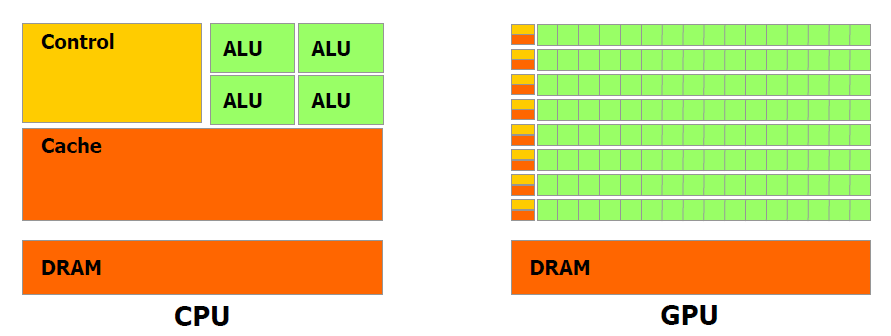
\includegraphics[width = \textwidth]{src/2Gpu/CPUGPU.png}
          \caption{Rozdíly využití čipu na CPU a GPU, převzato z \cite{CUDA programming g.}}
        \end{figure}\label{cpu vs gpu}

        Vidíme, že velkou část čipu CPU zabírá cache a kontrolní logika. Ty zajišťují několika ALU\footnote{Arithmetic Logic Unit} dostatečný přísun dat a instrukcí (např. pomocí hyper-threadingu a branch-prediction), lhostejno jak moc se program větví, nebo jak jsou data uspořádána v DRAM.

        GPU se naproti tomu skládá z několika samostatně funkčních vektorových procesorů -- tzv. SM\footnote{Streaming Multiprocesor} jednotek, z nichž každá má vlastní malou cache a z kontrolní logiky má naprosté minimum. Z toho plyne jednak jistá nutná disciplína při přístupu do DRAM, která je ale narozdíl od té na CPU lépe optimalizovaná na sekvenční čtení, a za druhé musíme běh programu přizpůsobit tomu, že GPU je po částech SIMD\footnote{Single Instruction Multiple Data}, respektive SIMT\footnote{Single Instruction Multiple Thread -- název pocházející od NVIDIA} -- narozdíl od vícejádrového CPU, které je plnohodnotné MIMD\footnote{Multiple Instruction Multiple Data}. Podrobný popis nejnovějšího SM z čipu \FERMI ~lze nalézt v \cite{Fermi}.

        Obecně můžeme říci (protože velká část čipu GPU je dedikována pro aritmetiku), že GPU je nejvíce vhodná pro aritmeticky intenzivní výpočty, tzn. mající vysoký poměr počtu aritmetických operací ku počtu přístupů do paměti.

    \subsection{Algoritmy vhodné pro GPU}

        Před paralelizací algoritmu pro GPU musíme tedy zvážit, zda to má vůbec smysl -- pro dosažení optimálního urychlení musí algoritmus v co největší míře splňovat následující body:
        \begin{itemize}
          \item rozložitelnost výpočtů na nezávislé části, které lze vykonávat paralelně (výsledek jedné nezávisí na výsledku ostatních)
          \item malý počet přístupů do paměti, nejlépe sekvenční/blokové
          \item podobný kód ve všech paralelních částech, minimální a předvídatelné větvení programu
        \end{itemize}

        Jak uvidíme, filtrování obrazu nesplňuje tyto body úplně (např. přístupy do paměti) -- kdyby splňovalo vše, tak se jím nemá příliš cenu zabývat -- ale dostatečně na to, abychom dosáhli použitelných výsledků.

\section{Pogramovací model CUDA a jeho HW implementace}

    \subsection{Úvod}
    Pro maximální efektivitu paralelizace vyvinula NVIDIA několikavrstvou dobře škálovatelnou strukturu s přímou návazností na svůj hardware. Nejmenší výpočetní jednotkou z pohledu programu je \emph{thread} (vlákno), který fyzicky běží na jednom CUDA-jádře v SM. Thready se sdružují do \emph{thread-bloků}, které běží na celém SM a mohou mít 1D, 2D, nebo 3D strukturu, podle toho jakého charakteru jsou zpracovávaná data. Poslední článek tvoří \emph{grid} běžící na celé GPU obsahující (zatím) nejvýše 2D strukturu thread-bloků. Z programu pak výpočty spouštíme pomocí volání \emph{kernelu} obsahujícího náš kód, kterému sdělíme v kolika thread-blocích má běžet, jakou mají mít strukturu v gridu, kolik threadů má být uvnitř thread-blocku a jak mají být uspořádány. To umožňuje ten samý kernel spouštět na různých zařízeních, protože sám hardware rozhoduje, jak jednotlivé výpočetní elementy mezi SM (a posléze CUDA-jádra) rozdistribuuje.

    \subsubsection{Úrovně přístupu}

    Na straně uživatele poskytuje NVIDIA dvě rozhraní: nízkoúrovňové CUDA Driver API a vysokoúrovňové CUDA runtime API, v současnosti ve verzi 4.0. Driver API poskytne uživateli totální kontrolu nad kartou výměnou za složitější a delší kód -- uživatel musí zajistit inicializaci zařízení, přesun dat a funkčních parametrů pro kernel na kartu a přesun a spuštění kernelu samotného. Rozhraní Driver API je v C a funkčně zhruba odpovídá OpenCL. Runtime API je rozšířením C, které umožňuje kernel napsat podobně jako funkci v C a při volání jí speciální syntaxí sdělit, kolik threadů a bloků chceme spustit. O inicializaci a vše ostatní se postará runtime. Nevýhodou Runtime API je, že jeden CPU proces nemůže používat více zařízení, což se ale nové verze snaží vylepšit.

    Mixování obou přístupů (např. právě kvůli použití více zařízení) se nedoporučuje, ale v rozumné míře možné je -- pravidla mixování stanovila až CUDA 4.0. V našem kódu používáme výhradně Runtime API, proto se dále budeme zabývat pouze jí.

    \subsubsection{Výpočetní schopnost}

    Tento termín bude dále v textu často používán. Výpočetní schopnost\footnote{Compute Capability} (VS) udává fyzickou verzi čipu -- všechna CUDA-enabled zařízení před architekturou \FERMI ~mají VS 1.x, čipy s touto architekturou 2.x. Různé VS se liší množsvím paměti, registrů, strukturou SM atd. Největší skok je samozřejmě mezi 1.x a 2.x. Podrobný popis rozdílů mezi VS je k dispozici v \cite[přílohy]{CUDA programming g.}. Pokud budeme dále uvádět konkrétní hodnoty, budou pro VS 1.0, pro kterou je kód primárně optimalizován. Pokud to bude důležité, bude v závorce uvedena hodnota pro VS 2.0. \note{-- na kartách s těmito VS budou totiž i počítány experimentální výsledky.}

    \subsection{Kernel}

    Runtime API nám dovoluje míchat kód pro CPU i GPU v jednom souboru, definici kernelu proto rozlišíme specifikátorem
    \Vr"\cy{__global__}" (příklad převzat z \cite{CUDA programming g.}).

    \begin{Verbatim}[commandchars = \\\{\}]
    // definice kernelu
\cy{__global__} \bl{void} MyVecAdd(\bl{float} *A, \bl{float} *B, \bl{float} *C)\{
    \bl{int} i = \cy{threadIdx}.x;
    C[i] = A[i] + B[i];
\}
    // volání kernelu v programu
    MyVecAdd<<<1,N>>>(A,B,C);
    \end{Verbatim}

    Při volání v příkladu specikujeme, že chceme jeden thread-blok a N threadů jako vektor, vektory A, B a C musí být při volání již připraveny v paměti karty. Po spuštění dostane každý thread (potažmo thread-blok) své ID, které je v kódu přístupné skrze read-only proměnnou \Vr"\cy{threadIdx}" (potažmo \Vr"\cy{blockIdx}") a umožní tak diferenciaci threadů. V kernelu tedy píšeme kód \emph{jediného threadu}, jehož konkrétní chování se po spuštění \emph{odvíjí od přiděleného ID námi definovaným způsobem}.

    \subsection{Hardwarová paralelizace, multithreading}

    Zde popíšeme, co se skutečně děje při spuštění kernelu na GPU. Přitom se omezíme pouze na jeden SM, protože všechny SM na kartě pracují zcela nezávisle a jakákoliv jejich synchronizace v rámci jednoho kernelu není možná.

    Po spuštění kernelu se bloky rozdistribuují mezi jednotlivé SM. Kolik bloků se vejde současně na jeden SM je dáno tím, kolik registrů a sdílené paměti blok spotřebuje -- tyto hodnoty jsou pevně stanoveny při spuštění kernelu. Pokud se na SM nevejde ani jeden blok, spouštění kernelu selže. V opačném případě hardware umístí na každý SM maximální možný počet bloků, zbývající bloky budou čekat na uvolnění některého SM.

    SM má však pouze 32 CUDA-jader, tzn. bloky běží současně pouze virtuálně. Důvod tohoto \bq přesycení\eq~ spočívá v \emph{překrytí latencí} způsobených například čtením a zápisem do paměti: pokud například nějaký \emph{warp} (což je 32 synchronně běžících threadů na oněch 32 CUDA-jádrech) čeká na načtení operandů z paměti, může mezitím jiný warp (protože má např. proměnné připravené v registrech) provádět výpočty -- i když je to třeba warp z jiného bloku. Rychlé přepnutí warpů\footnote{tzv. context switch} je umožněno tím, že thread na GPU je narozdíl od toho na CPU velmi jednoduchá struktura a multithreading na GPU je dělán hardwarově. Z toho vyplývá jisté omezení na maximální počet bloků a threadů/SM (přesná čísla lze nalézt v \cite{CUDA programming g.}). Ve většině případů ovšem dříve vyčerpáme registry, nebo sdílenou paměť, než se dostaneme k tomuto stropu.

    Pro efektivní využití výpočetních jednotek je nutné, aby pokud možno všechny thready v jednom warpu prováděly stejný kód, neboť celý warp zvládá naráz vykonávat pouze jedinou instrukci (dvě instrukce pro dva 16threadové půlwarpy pro VS 2.x), což odpovídá filozofii SIMD. Všechna větvení kódu by tedy měla být směřována na hranice warpů, tzn. mezi 32 po sobě jdoucích threadů. V opačném případě bude warp rozdělen na části se stejnou posloupností instrukcí a ty budou zpracovány sériově.

    \subsection{Práce s pamětí}

    Jak jsme zmínili v úvodu kapitoly, paměťové zdroje karet jsou poměrně omezené a vhodné zacházení s pamětí je tak prvním předpokladem pro to, aby paralelizovaný algoritmus dosáhl optimálních výsledků. Vývoj jde ale v této oblasti hodně dopředu a architektura \FERMI ~má již paměti mnohem více a lépe strukturované.

    \subsubsection{Registry}

    Jsou velmi podobné klasickým registrům na CPU a jsou zdaleka nejrychlejší pamětí dostupnou pro thread -- proto se do nich ukládají všechny lokální proměnné, kromě polí. Karty s VS 1.x mají 8192 (1.0) až 16384 (1.3) registrů/SM, VS 2.x má 32768 registrů/SM. V kódu není třeba je nějak značit, většina lokáních proměnných (viz dále) se do nich sama uloží.

    \subsubsection{Sdílená paměť}

    Jedná se o paměť zabudovanou v každém SM, dostupnou na úrovni bloku a umožňující komunikaci threadů v bloku. Jako de facto manuální (a pro VS 2.x i částečně automatická) cache je přímo na čipu GPU a tudíž je poměrně rychlá. Pro optimální rychlost je rozdělena do 32 banků tak, že thready (jednoho warpu) čtoucí 32 po sobě jdoucích položek z pole v této paměti přistupují každý do jednoho banku a celé čtení je možné vyřídit jako jedinou operaci.

    V kódu statické pole pevné délky ve sdílené paměti deklarujeme pomocí identifikátoru \Vr"\cy{__shared__}" -- takto je definováno jedno pole pro celý blok (obyčejná proměnná bez identifikátoru by byla vytvořena pro každý thread) a všechny thready bloku do něj mají přístup. Synchronizace čtení a zápisu je ponechána na uživateli.

    Pole ve sdílené paměti je možné alokovat i dynamicky z CPU: v kernelu ho deklarujeme pomocí identifikátoru \Vr"\bl{extern}":
    \begin{Verbatim}[commandchars = \\\{\}]
\bl{extern} \cy{__shared__} \bl{datovýtyp} jménopole[];
    \end{Verbatim}
    Při spouštení kernelu poté pomocí třetího parametru {\tt Ns} zadáme, kolik chceme navíc (kromě režie) alokovat bytů sdílené paměti pro blok.
    \begin{Verbatim}[commandchars = \\\{\}]
MyKernel<<<1,N,Ns>>>(parametry);
    \end{Verbatim}
    Námi deklarované pole se naváže na začátek této alokované paměti. Nevýhodou je, že při deklaraci více dynamicky alokovaných polí budou všechny začínat na začátku této paměti (jako v unii) a případné rozdělení pole musíme tedy provést ručně pomocí ukazatelů a offsetů. Dynamická alokace přímo z kernelu není (principiálně) možná. Životnost dat ve sdílené paměti je stejná jako životnost bloku.

    \subsubsection{Globální paměť}

    Největší paměť na GPU (jednotky GB). Protože není fyzicky umístěna na čipu, přístup do ní je velmi pomalý -- řádově stovky taktů -- nicméně je optimalizová pro sekvenční čtení a zápis z GPU. Hardware totiž umožňuje přístup pouze po 128-bitových blocích. Pokud nechceme, aby došlo ke zpomalení, je nutné, aby všechny thready v jednom warpu (a tudíž vykonávající stejnou instrukci) přistupovaly do co nejmenšího počtu těchto bloků, ideálně do jednoho. Tím dojde k tzv. \emph{sdruženému přístupu}\footnote{Coalesced access} a všechny přístupy threadů do sousedících míst v paměti mohou být obslouženy v rámci jediného požadavku. Konkrétní způsob (omezení), jak mohou thredy k paměti v bloku přistupvat je závislý na výpočetní schopnosti karty a jeho popis lze nalézt v \cite{CUDA programming g.}.

    Alokace, čtení a zápis do této paměti je možný i z CPU (samozřejmě na jiné bázi), data zapsaná tímto způsobem mají pak životnost stejnou, jako aplikace.

    V kódu se ukazatel do globální paměti neliší od jiných ukazatelů\footnote{K dispozici je i \bq novější\eq ~obecný typ ukazatele do globální paměti {\tt DevicePtr*}, který vyžadují nekteré fukce. Spíše jde ale o snahu nějak data na CPU a GPU formálně oddělit. Kód využívající tento typ ukazatele se nám však nepodařilo zprovoznit. Se starší verzí jsou však dobré zkušenosti.}, postup zkopírování dat na GPU je následující:
    \begin{enumerate}
      \item Vytvoření běžného ukazatele na požadovaný typ
      \item Přiřazení ukazatele k alokovanému poli v globální paměti pomocí {\tt CudaMalloc(...)}
      \item Zkopírování dat z pole v RAM na GPU pomocí {\tt CudaMemcpy(...)}
      \item Ukazatel se předá kernelu přes obyčejný parametr
    \end{enumerate}
    Na CPU nelze ukazatel do globální paměti dereferncovat přímo, na GPU to však lze bez jakýchkoliv omezení.

    Samotnou alokaci opět není možné provádět z GPU, pokud však využívá thread větší statické pole jako lokální proměnnou, nebo tolik proměnných, že se nevejdou do registrů\footnote{tzv. Register spilling}, uloží se přebytek v \emph{lokální paměti}. Lokální zde znamená pouze omezení životnosti dat, data jsou ve skutečnosti uložena do globální paměti -- se všemi nevýhdami, které z toho plynou. Z tohoto důvodu je dobré se použití lokální paměti jakýmkoliv způsobem vyhnout.

    \subsubsection{Konstantní paměť}

    Konstatntní paměť je 64 KB velká část globální paměti s vlastní cache, tudíž je celkem rychlá a vhodná pro objemné konstanty. Je přístupná z CPU pro čtení i zápis, dynamická alokace není možná ani z CPU. Z GPU lze paměť pouze číst -- proto konstatní.

    V kódu se pro tuto paměť používá identifikátor \Vr"\cy{__constant__}" a proměnné s tímto identifikátorem musíme chápat spíše jen jako pojmenování místa v konstantní paměti karty. Poněkud nepříjemné je, že z tohoto důvodu musí být všechny tyto proměnné v kódu definovány jako globální a na úrovni souboru. Nesmí být tedy schovány do jakéhokoliv prostoru jmen, ani do třídy (byť jako statické), jak je zvykem ve slušném \Cpp kódu. Hodnoty do proměnných (polí) v konstantní paměti přesuneme z RAM pomocí {\tt CudaMemcpyToSymbol(...)}.

    \subsubsection{Texturová cache}

    Texturová paměť někdy představuje rychlejší alternativu k čtení (\emph{nikoliv zápisu}) z globální paměti. Část dat můžeme totiž prohlásit za \emph{texturu}, což znamená, že data budou každým SM částečně cacheována (pokud je textura větší než cache). Velikost cache je 6-8 KB/SM, přitom hardware sám odhaduje, která data bude chtít program načíst a ty do ní přesune\footnote{tzv. Texture fetching}. Pokud jsou požadována data, která nejsou v cache k dispozici\footnote{tzv. Cache miss (v opačném případě Cache hit)}, jsou normálním způsobem načtena z globální paměti. Používání textur je tedy výhodné, pokud bloky potřebují relativně malé a dobře definované kousky dat, které se do cache vejdou celé.

    Protože se jedná o činnost hodně blízkou klasické grafice, je v kódu citelně znát odkaz grafického API. Před použitím textury musíme definovat referenci na texturu (opět globální stejně jako konstantní proměnné) a ještě na CPU ji svázat s požadovanými daty pomocí {\tt cudaBindTexture(...)}. Obě operace potřebují značné množství parametrů (potřebných při používání textur pro původní účel), jejich popis lze nalézt v~\cite{CUDA programming g.}. Číst z takto připravené textury je na GPU možné pomocí funkce {\tt texXDfetch(...)} ({\tt X} je 1,2,3).

    VS 2.x již umožňuje volitelné cacheování globální paměti za použití části sdílené paměti, textury ale stále představují průchozí alternativu. Nezaberou totiž sdílenou paměť a využijí několik cenných KB paměti jinak nepoužívané.

    \subsection{Možnosti synchronizace}

    Synchronizace threadů je nutná pro jakoukoliv jejich kooperaci mezi sebou. CUDA umožňuje synchronizaci na úrovni bloku pomocí instrukce \Vr"\cy{__syncthreads()}", která zastaví běh threadů, dokud všechny v jednom bloku tuto instrukci nezavolají. To se hodí například při práci se sdílenou pamětí, kdy chceme zajistit, aby z ní všechny thready začaly číst až poté, co do ní budou (např. menším počtem threadů) zapsána relevantní data.

    CUDA navíc poskytuje i několik speciálních instrukcí čistě pro synchronizaci přístupů do paměti (viz \cite[přílohy]{CUDA programming g.}), což je jediná možnost, jak částečně synchronizovat thready v celé aplikaci -- ovšem za cenu výrazného zpomalení (poruší se přepínání bloků na SM kvůli překrývání latencí).

% v implementaci chceme už jen popisovat optimalizace, programming model už musí být hotový 

    \chapter{Implementace v CUDA}
        % Kernel
        % Paměťové optimalizace
        % Instrukční optimalizace
        % ??

        % -*-coding: utf-8 -*-

Před tím, než se podíváme na implementaci konkrétních filtrů, probereme některé optimalizace, které budeme často používat. Mnoho z nich je velmi obecných a používají se pro jakýkoliv kód spuštěný na GPU. Naopak některé optimalizace popisované v \cite{CUDA programming g.}, \cite{CUDA best practices} v našem kódu nepoužijeme, neboť pro nás nejsou vhodné. Pro jejich podrobnější popis odkažme čtenáře na zmíněnou literaturu.

\section{Použité optimalizace}

    Dvě hlavní třídy optimalizací se týkají optimalizace práce s pamětí a toku instrukcí. V našem případě (a částečně obecně) má vyšší prioritu optimalizace paměti. Přístup do paměti totiž vykazuje narozdíl od vykonávání instrukcí vysokou latenci a náš kód do ní potřebuje přistupovat, v poměru k počtu aritmetických operací, velmi často\footnote{kód je tzv. memory-bound}.

    \subsection{Optimalizace paměti}

        Následující přehled ukazuje různé běžné paměťové operace seřazené od nejpomalejších:
    \begin{itemize}
      \item Přesun dat z CPU na GPU a zpět
      \item Čtení a zápis do globální paměti GPU
      \item Čtení z texturové cache a dalších cache
      \item Čtení a zápis do sdílené paměti
      \item Čtení a zápis do registrů
    \end{itemize}

        \subsubsection{Tok dat mezi CPU a GPU}

        Pro jeho slouží celá řada typů RAM optimalizovaných pro konkrétní typy operací (CPU pouze zapíše, GPU pouze čte apod.), stále se však jedná o komunikaci přes PCI Express a ta bude proti komunikaci uvnitř karty vždy řádově pomalejší. Nejefektivnější, a pro náš případ nejproveditelnější optimalizací, je redukce těchto přenosů na nezbytné minimum, což není velký problém -- zpracovávaný obraz (obrazy) stačí na začátku přesunout na GPU, všechny mezivýsledky, které nepotřebujeme, ukládat tamtéž a pouze výsledek poslat zpět.

        \subsubsection{Čtení z globální paměti}\label{globální pam opt}

        V našem případě sice čteme souvislé bloky paměti, avšak díky závislosti na uživatelské volbě masky a rozměrech obrázku je nemožné zajistit, aby byl čtený blok \emph{zarovnán} na 128 bitů, jak to vyžaduje VS 1.x, pro niž byl kód optimalizován. Filtry však pracují s pamětí velmi extenzivně a dochází k \emph{opakovanému čtení} ze stejného umístění (jeden voxel se promítne do výsledku mnoha okolních), na což je globální paměť zcela nevhodná. Díky malému rozsahu dat zpracovávaných jedním blokem tedy používáme ke čtení výhradně texturovou cache (1D, namapovanou na celý obraz), případně kombinovanou s kopírováním celého bloku dat do sdílené paměti.

        Zápis je bezproblémový, protože se jedná vždy jen o jednu hodnotu za thread (nebo skupinu threadů) a tudíž jsou přístupy threadů s po sobě jdoucími \Vr"\cy{threadIdx}" automaticky sdružené.

        \subsubsection{Konstantní paměť}

        Konstantní paměť používáme k uložení všech dlouhodobě neměnných dat -- všech předpočítaných geometrických veličin a část dat masek. U masek neukládáme {\tt wList}, jelikož jeho velikost je proměnná na velké škále a definováním vysoké horní hranice bychom rychle konstatní paměť vyčerpali. {\tt wList} je ovšem na začátku každého kernelu manuálně zkopírován do sdílené paměti pomocí makra {\tt SE\_TO\_SHARED}.

        \subsubsection{Optimalizace registrů}

        Vzhledem k tomu, že algoritmy pro většinu filtrů jsou poměrně jednoduché, výsledné kernely jsou poměrně malé a na jeden SM se nám vejde velký počet bloků (nebo alespoň threadů), což je ideální, protože se dobře překryjí paměťové latence. Bloky ale bohužel nejsou paměťově tak malé, aby se uplatnilo hardwarové omezení a zvyšování jejich počtu na jednom SM tak bude střídavě narážet na fyzické omezení množsví sdílené paměti (probráno u konkrétních filtrů) a hlavně registrů\footnote{pro představu naše thready spotřebují zhruba 11-23 registrů. To pro VS 1.x (8192 registrů/SM) odpovídá 744-356 threadů/SM, což ještě nenaráží na fyzickou hranici 768 threadů/SM (VS 1.1)}.

        Pro snížení počtu použitých registrů můžeme udělat několik věcí:
        \begin{itemize}
          \item Recyklace proměnných -- proměnné, jejichž obsah není aktuálně potřeba použít pro dočasně např. jako inkrementální proměnné v cyklech.
          \item Řízená výměna rychlosti za menší počet využitých registrů změnou algoritmu (v optimalizaci kompilátoru by ale měla být pořád zapnutá optimalizace na rychlost).
          \item Uložení méně potřebných dat do sdílené paměti, případně uložení konstantních maker do konstantní paměti -- zde je nutné experimentovat, \emph{celková} rychlost může i při větší hustotě bloků/SM klesnout.
          \item Opatrné používání C příkazu \Vr"\bl{goto}" při vyskakování z mnoha cyklů naráz nám také může ušetřit jednu kontrolní proměnnou.
        \end{itemize}

        Pro další experimentování nám pomůže sledování obsazenosti SM pomocí CUDA Occupancy Calculator\footnote{přehledný excelový program dodávaný s CUDA SKD}, kde můžeme zjistit, na jakou z výše zmíněných hranic právě narážíme. Zde můžeme například zjistit, že na SM se již další blok nevejde a tak naopak navýšit počet registrů a zvýšit tak rychlost. Mírnou nevýhodou je, že tyto jemné optimalizace už jsou zcela závislé na konkrétní VS, protože každá má jiné množství registrů a sdílené paměti.

        Další nepříjemností, co se týče uvolňování registrů jsou systémové proměnné typu \Vr"\cy{threadIdx}" a \Vr"\cy{blockIdx}", které zřejmě\footnote{podle provedených experimentů}\note{podívat se do PTX??} v registrech zůstávají, byť je občas potřebujeme jen na začátku kernelu. Navíc se ani nemohou účastnit recyklace, protože do nich není možné zapisovat. Z tohoto důvodu je při extrémní minimalizaci počtu registrů praktické volit dimenzionalitu gridu a bloku co nejmenší (s tím je ale nutné počítat od začátku).

    \subsection{Optimalizace běhu kernelu}

    Následující sekce obsahuje několik dalších optimalizací, které se při experimentování s kernely osvědčily. \note{nejsou už tolik univerzální?}

        \subsubsection{Synchronizace}

        Několik poznámek k instrukci \Vr"\cy{__syncthreads()}":
        \begin{itemize}
          \item Rozhodně s nimi šetřit, neboť nejsou časově nejlevnější -- sice zaberou jen 8 taktů \cite{CUDA programming g.}, ale jak jsme zmiňovali, přeruší cyklus překrývání latencí, což může způsobit značné zpomalení.
          \item Pokud se program větví, všechny větve musí obsahovat \emph{stejný počet} \Vr"\cy{__syncthreads()}", protože GPU k prohlášení bloku za synchronizovaný stačí, aby každý thread dorazil k \emph{nějaké} synchronizační instrukci, tzn. nemusí to být u všech threadů ta samá. Porušení tohoto vede ve většině případů k pádu programu.
          \item Speciálním případem předchozího je, že jeden thread zavolá \Vr"\bl{return}" a ostatní na něj při synchronizaci marně čekají (až do resetu GPU).
        \end{itemize}
        V našich memory-bound kernelech se tedy budeme požití \Vr"\cy{__syncthreads()}" vyhýbat, pokud to půjde.

        \subsubsection{Větvení programu}\label{větvení}

        Z předchozího je jasné, že větvení je nejlépe omezit pouze na hranice warpů, pokud už nejde zcela vynechat. Je logické, že nejvíce musíme větvení optimalizovat v nejvytíženějších částech kódu. Příklad:
        \begin{itemize}
        \item Podmínku na začátku kódu ověřující, zda má thread ještě vůbec nějaká data ke zpracování, většinou vynechat nelze, ale také nijak nezhoršuje výkon -- dotkne se pouze několika posledních waprů v posledním bloku. Toto se týká obecně podmínek rozumně závisejících pouze na ID threadu (\Vr"\cy{threadIdx}",\Vr"\cy{blockIdx}").
        \item Cyklus obsahující několik (krátkých, nejlépe jednoinstrukčních) podmínek závislých na vnitřních proměnných naproti tomu bude generovat poloprázdné warpy po dobu běhu celého kernelu a zde je na místě pokusit se větve odstranit.
        \end{itemize}
        Jeden z případů druhé skupiny, kde se dá větvení zcela odstranit je následující:
        \begin{Verbatim}[commandchars = \\\{\}]
\bl{if}(x<y) z++;
        \end{Verbatim}
        lze ekvivalentně přepsat na
        \begin{Verbatim}[commandchars = \\\{\}]
z += (x<y);
        \end{Verbatim}
        kde se spoléháme na normu\footnote{nevíme, jeslti je \emph{zaručeno}, že ji kompilátor dodržuje, nebo zda je to machine-dependent záležitost -- nutno vyzkoušet}, že podmínka má hodnotu 1, pokud platí a 0, pokud ne. Pokud se takovéto podmínky nalézají ve vytížené části kódu, může být urychlení znatelné. Zdá se totiž, že syntaxi s \Vr"\bl{if}" kompilátor nezvládne zoptimalizovat a vytvoří dvě větve (výsledek podmínky použije pro podmíněný skok), zatímco v druhém případě mu explicitně říkáme, jak má výsledek podmínky použít. Ze stejných důvodů je výhodné používat ternární operátor \Vr"?" kdekoliv je to možné.

        Narozdíl od CPU není vhodné tvořit z několika složitých po sobě jdoucích podmínek stromy obsahující jednodušší podmínky -- thread sice musí prozkoumat v průměru méně podmínek, aby stromem prošel, vznikne tím ovšem hodně \emph{divergentních threadů} (po cestě, kterou se vydali nejdou skoro žádné další thready z warpu) a výpočty budou serializovány (způsobí vytvoření mnoha řídce obsazených warpů). Ponecháme-li složité podmínky v kódu volně za sebou, bude sice vyhodnocení samotné podmínky trvat déle, ale bude vykonáno všemi thready naráz, protože ty se mezi podmínkymi synchronizují a tudíž bude kód ve výsledku ryhlejší.
        \begin{Verbatim}[commandchars = \\\{\}]
// rychlejší varianta
\bl{if}(...) && (...)\{
...     // dvě (silné) větve
\}
    // zde se thready synchronizují
\bl{if}(...) && (...)\{
...     // dvě (silné) větve
\}

// pomalejší varianta
\bl{if}(...)\{
    \bl{if}(...)\{
    ...      // tři větve
    \}\bl{else if}(...)\{
    ...
    \}
\}
        \end{Verbatim}

\section{Implementace filtrů na GPU}

    Zde se konečně dostáváme ke popisu kernelů provádějících filtraci. Nyní v bodech probereme, co máme před začátkem vlastní filtrace k dispozici a co musíme při psaní kódu zohlednit:
    \begin{itemize}
      \item Každý vstupní voxel chceme zpracovávat jedním threadem, nebo skupinou threadů (opak by šel proti filozofii paralelizace).
      \item 3D data a {\tt wList} z masky jsou na GPU v globální paměti uložena ve stejném formátu jako na CPU.
      \item Kernelu je předána reference na texturu, která byla svázána se zpracovávanými daty.
      \item V konstantní paměti GPU máme připravenou veškerou potřebnou geometrii a konstatní data masek.
      \item Po inicializační části threadu máme k dispozici {\tt wList} použité masky ve sdílené paměti a v proměnné {\tt thread} index zpracovávaného voxelu vypočtený z ID threadu.
    \end{itemize}

    Konkrétní kód inicializační části kernelu zde popisovat nebudeme, neboť její průběh není přiliš podstatný a navíc je kód díky optimalizacím (rychlost, recyklace proměnných) lehce nepřehledný. Nyní již k jednotlivým filtrům.

    \subsection{Morfologické filtry}

    Jejich implementace je opět triviální: thread v cyklu načítá z textury podle {\tt wList} hodhoty okolních voxelů a z nich vybere minimum (eroze), maximum (dilatace), nebo oboje (detekce hran). Vzhledem k velkému množství přístupu do paměti ku počtu jiných operací (jedna, nebo dvě podmínky) se u těchto filtrů nedaří zcela překrýt paměťové latence. To má za následek, že v případě detekce hran je přidání druhé podmínky (jedna hledá maximum, druhá minimum) \bq zdarma\eq, neboť jinak by SM stejně nic nedělal a čekal na paměť. Množství přístupů do paměti je ovšem u detekce hran \emph{stejné}, jako u dilatace a eroze.

    Díky tomu ve výsledcích uvidíme, že detekce hran má takřka dvojnásobné relativní zrychlení vůči CPU (kde se podmínka navíc samozřejmě projeví), než dilatace, nebo eroze. U nich tedy má smysl uvažovat o snížení paměťových latencí. To by se dalo udělat například zkopírováním bloku zpracovávaných dat do sdílené paměti -- pro maximální efektivitu to však vyžaduje poměrně komplikovanou přestavbu kódu, včetně přepočítání masek a jiné režie, takže jsme od dalších optimalizací nakonec upustili.

    \subsection{Medián a BES}

    Součástí těchto filtrů je částečné třídění pole. V současnosti existuje spousta literatury popisující paralelizaci známých třídících algoritmů, jako quicksort, mergesort, bitonic sort apod., které se však zaměřují na třídění obřích polí (10$^6$ až 10$^9$ prvků) a zřídka bývají efektivní pro malá pole. V našem případě však potřebujeme paralelně setřídit \emph{mnoho malých} polí, a to nejlépe při malé spotřebě sdílené paměti, což hardwaru umožní přidělit více bloků na jedno SM a lépe tak překrýt latence.

    Pro malé velikosti polí (destíky prvků) jsou obecně výhodnější \bq hloupější\eq ~\OOO($n^2$) algoritmy, protože mají oproti složitějším algoritmům velmi malou režii. Při použití na GPU na ně navíc klademe požadavek, aby jejich průběh byl pokud možno nezávislý na vstupních datech (co nejméně větví, nebo alespoň stejně dlouhé) -- to zamezí přílišnému rozdrobení warpů, jejich serializaci a následnému zpomalení. Jako vítěz se při těchto požadavcích jeví algoritmus zapomětlivého třídění \cite{Forgetful}.

        \subsubsection{Zapomětlivé třídění}

        Buď \textbf{medián} \kk-tým prvkem v setříděném poli (\kk-tým a (\kk-1)-ním pro sudou délku pole), princip pro nalezení mediánu je následující:
        \begin{enumerate}
          \item Z nesetříděného pole vyberme libovolně \kk$+1$ prvků (nejjednodušeji od začátku pole).
          \item Mezi vybranými prvky najděme maximum a minimum a ty zahoďme.
          \item Do výběru přidejme jeden prvek z nesetříděného pole, který jsme ještě nevybrali.
          \item Opakujme kroky 2. a 3. dokud nezbyde pouze jeden prvek (dva pro případ sudé velikosti pole), ten je hledaným mediánem.
        \end{enumerate}

        Při hledání se tedy pole neustále zmenšuje, až zbyde pouze medián. Navíc nepotřebujeme současně celé pole, ale pouze něco přes polovinu, což kvůli latencím umožní zvýšit rychlost až dvakrát (!) oproti algoritmům využívajícím celé pole. Algoritmus je jistě \OOO($n^2$) -- počet hledání maxim a minim je roven součtu aritmetické řady. Také je jasné, že algoritmus se větví pouze při podmínkách nutných k nalezení maxima a minima (lépe to s comparison-based algoritmem nejde). Jako nejlepší \note{VYZKOUŠET DÁT JEN IF}

        Nyní dokažme, že algoritmus nikdy nezahodí medián -- budiž počet prvků v poli lichý, pro sudý to platí obdobně:

        V prvním kroku zaručujeme, že maximum i minimum budou jistě nad a pod hodnotou mediánu (ať už on sám je vybrán, nebo ne), protože vybraných prvků je \bq moc\eq ~-- nejhorší možné výběry ukazuje obrázek~\ref{obr forgetful}.
        \begin{figure}[h]\label{obr forgetful}
        \begin{center}
          \includegraphics[width = 0.75\textwidth]{src/4Implementace/forgetful.pdf}
          \caption{Nejhorší výběry při setříděném poli, modrá značí medián}
          \end{center}
        \end{figure}
        Vyhozením minima a maxima tedy o medián nepřijdeme. Uvidíme, že toto platí v každém dalším kroku:
        \begin{enumerate}
          \item Medián je mezi vybranými prvky:
            \begin{enumerate}
                \item Po zahození maxima a minima je medián stále uvnitř výběru (není minimem ani maximem z toho, co zbylo): při dalším kroku nebude zahozen
                \item Po zahození maxima a minima je medián (BÚNO) maximum ze zbytku: hodnota přidaná z ještě nesetříděných bude nutně větší než medián, neboť \emph{všechny} menší již ve výběru jsou (viz obrázek~\ref{obr forgetful}). Tudíž při dalším zahazování medián opět zůstane ve výběru.
            \end{enumerate}
          \item Medián není mezi vybranými prvky, ale je mezi ně přidán po zahození maxima a minima: ve výběru je příliš mnoho prvků, a tak všechny nemohou být (BÚNO) menší než přidávaný medián a ten tudíž nebude v dalším kroku maximem.
        \end{enumerate}

        Zapomětlivé třídění lze jednoduše modifikovat pro \textbf{BES} filtr: Na začátku stačí vzít tolik hodnot, abychom zajistili, že i první a třetí kvartil budou \emph{uvnitř} výběru (viz obrázek~\ref{obr forget BES}), poté provádíme
        \begin{figure}[h]\label{obr forget BES}
        \begin{center}
          \includegraphics[width = 0.75\textwidth]{src/4Implementace/forgetfulBES.pdf}
          \caption{Nejhorší výběry při setříděném poli, BES, modrá značí kvartily}
          \end{center}
        \end{figure}
        klasické zapomětlivé třídění. Po přidání poslední nesetříděné hodnoty je jasné, že nalezené maximum a minimum odpovídá třetímu a prvnímu kvartilu. Po jejich zapamatování dále již maxima a minima pouze vyhazujeme (nemáme co přidávat), dokud nezbyde medián. Argumentace správnosti je obdobná, jako v předchozím případě.

        Úspora paměti je v tomto případě menší -- limitně čtvrtina -- i tak má však algoritum velmi slušné výsledky.

    \subsection{Hodges-Lehmannův medián a WBES}

    Protože jsou tyto fitry postavené na Walshově seznamu (který na začátku paralelně vytvoříme), je tříděné pole již poměrně velké (stovky prvků). Kvůli tomu nám při přístupu jeden thread/jedno pole radidně klesne vytížení SM, protože se do sdílené paměti se vejde málo polí, a navíc se projeví pomalost \OOO($n^2$) algoritmů. Pro přístup pole/blok\footnote{což je také minimální hranice pro použití sofistikovanějších algoritmů} je zase pole příliš malé -- idelální je mnohonásobek velikosti bloku, zde máme v praxi něco kolem dvojnásobku.

    Jako kompromis jsme zvolili přístup pole/warp (nebo obecně skupina threadů) a použití velmi naivního algoritmu: pro každý prvek pole jednoduše spočítáme, kolik hodnot je ostře menší a ostře větších než tento prvek a na jejich základě určíme, zda je daný prvek mediánem (nebo libovolným jiným \kk-tým prvkem). Algoritmus má sice zcela jasně složitost \OOO($n^2$), ale dá se pro GPU výborně optimalizovat; popišme nyní jeho implementaci (popis jednoho warpu -- 32 threadů):
    \begin{enumerate}
      \item Ze vstupních dat vytvoříme ve sdílené paměti Walshův seznam (WS).
      \item Každý thread si zapamatuje jeden z 32 prvků ze začátku WS.
      \item V cyklu porovnává každý thread zapamatovaný prvek postupně se všemi prvky WS, počítá ostře menší a ostře větší prvky. Thready přitom postupují synchronně a v každém kroku je porovnávaný prvek pro všechny thready stejný.
      \item Každý thread ověří, zda nenalez medián (případně jiný potřebný \kk-tý prvek), pokud ano, zapíše ho paměti.
      \item Pokud byly nalezeny všechny hledané prvky, warp už jen počká na konec celého bloku.
      \item V opačném případě načte warp dalších 32 prvků z WS a pokračuje na krok 3.
    \end{enumerate}
    \begin{figure}[h]
    \begin{center}
      \includegraphics[width = 0.75\textwidth]{src/4Implementace/scansort.pdf}
      \caption{Schéma algoritmu pro Hodges-Lehmannův medián a WBES}
    \end{center}
    \end{figure}

    Z definice mediánu (\ref{def median}) je zřejmé, že daný prvek je medián, právě když platí následující dvě nerovnosti ($c$ je délka pole, $p$ označuje množství napočtené při porovnávání):
    \begin{align}
      p_{(<)} < \Big\lfloor\frac{c+1}{2}\Big\rfloor \notag \\
      p_{(>)} < \Big\lceil\frac{c+1}{2}\Big\rceil \notag
    \end{align}
    Obdobné nerovnosti lze stanovi i pro jakýkoliv jiný \kk-tý prvek.

    Výhodou této imlementace je, že v časově nejnáročnější části (krok 3.) se algoritmus díky použití optimalizace~\ref{větvení} vůbec nevětví a navíc minimálně přistupuje do paměti (načtení pouze jediného prvku pro celý warp). Navíc díky zapisování nalezených hodnot může algoritmus skončit ještě dříve, než porovná prvky \emph{všechny} prvky, což mírně sníží konstantu u časové náročnosti.

    Je zřejmé, že popsaný algorimus lze použít jak pro H-L mediá, tak pro WBES -- vše záleží pouze na volbě podmínek v kroku 4.

    \note{GPU je někde mezi tím, že čas výpočtu je více závislý na celkovém počtu uzlů stavového stromu, než na délce jeho cest ?!} 

    \chapter{Výsledky}
        % volba masky
        % Testovací data
        % Testovací sestava
        % Urychlení vůči CPU

        % -*-coding: utf-8 -*-

Připomeňme, že nás nyní \emph{nezajímá} rychlost konvergence algoritmů, nebo přesněji veličina $\frac{\text{doba konvergence}}{\text{počet vyčíslení účelové funkce}}$. Ta je velmi závislá na úloze, nastavení parametrů algoritmu a~paralelizace ji -- až na zmíněný efekt superlineárního urychlení -- příliš neovlivní. \emph{Nyní nás zajímá doba výpočtu jednoho kroku algoritmu (jedné generace) a zkrácení této doby při použití GPU}.

\section{Příprava testování}
\subsection{Hardware}

Hardwarová sestava pro testy byla následující:

\begin{table}[h]
    \begin{center}
    \begin{tabular}{lcc}
      \toprule
      & CPU & GPU \\
      \midrule
      Název & AMD Phenom$^\mathrm{TM}$ II X4 945 & NVIDIA GeForce GTX 460 \\
      Výpočetní jednotky & 4 (využita 1) & 336 (7 SM $\times$ 48 CUDA-jader) \\
      Frekvence & 800 MHz & 675 MHz \\
      Výpočetní schopnost & --- & 2.1 \\
      Cache & 2 MB L2 & --- \\
      RAM/DRAM & 4 GB & 768 MB GDDR3 \\
      FSB & ? & 1800 MHz \\
      \bottomrule
    \end{tabular}
    \caption{Testovací sestava}
    \end{center}
\end{table}

Je nutné podotknout, že ani CPU, ani GPU zdaleka nejsou na špičce současných produktových řad. Při paralelizaci na dnešních nejvýkonnějších CPU (Intel Core i7 -- 4 jádra, 8 vláken, 3GHz) bychom mohli dosáhnout proti testovanému CPU teoretického urychlení cca $30\times$. Urychlení současné nejvýkonnější GPU (Nvidia GTX690 -- 3072 jader, 915Mhz, dvojnásobná rychlost zpracování instrukcí) oproti testované by se mohlo pohybovat kolem $25\times$. Technologický trend by tedy naše výsledky neměl výrazně vychýlit ve prospěch CPU.

\subsection{Testované algoritmy a použité účelové funkce}
Testovali jsem algoritmy náhodná střelba (RS), genetická optimalizace (GO), a simulované žíhání (SA). Jako účelové funkce jsem zvolili sférickou De Jongovu funkci č. 1 a problém \emph{sudoku}. De Jongova funkce č. 1 vypadá následovně:
\[
f_{DJ} = \sum_1^n x_i^2,
\]
kde $x_i$ je $i$-tá složka kandidáta. Počet dimenzí ($n$) byl nastaven na 5. Jednalo se tedy o~jednoduchý problém s nízkou dimenzí, kde by měla vyniknout kvalita paralelizace zbylé logiky algoritmu.

Problém \emph{sudoku} má simulovat hledání přípustného řešení za pomocí penalizační funkce. Úloha má 81 dimenzí, povolené hodnoty jsou celá čísla z $[1,9]$. Velikost penalizace odpovídá počtu konfliktů v řádcích, sloupcích a ve čtvercích. Úloha byla zvolena jako příklad většího, algoritmicky náročnějšího, avšak plně paralelizovatelného problému.

\subsection{Parametry algoritmů}

Uživatelské parametry u algoritmů byly zvoleny následovně:
\begin{itemize}
  \item RS: Nemá parametry.
  \item GO: Pravděpodobnost křížení: 50\% , pravděpodobnost mutace: 90\%, rozptyl mutace $\sigma^2 = 1$. Na rychlost výpočtu má vliv pouze pravděpodobnost křížení a mutace, neboť ta určuje, kolik dat se bude muset zpracovat.
  \item SA: Počáteční teplota: $10^6$, rozptyl mutace $\sigma^2 = 50$. Žádný z těchto parametrů však příliš neovlivňuje rychlost výpočtu.
\end{itemize}

U algoritmů jsme měřili, jak dlouho trvá spočítat 100 generací\footnote{Než algoritmus zkonverguje na reálném problému, trvá to běžně tisíce generací}. Na GPU byl spuštěn pro 20 různých konfigurací velikosti populace (32, 64, 128, 256, 512) a počtu paralelních populací (1, 10, 100, 1000). Na CPU jsme testovali jen 5 konfigurací se stejnými velikostmi populace, avšak pouze s jednou \bq paralelní\eq~ populací. U GO byla velikost potomstva nastavena vždy na dvojnásobek velikosti populace. V každé konfiguraci byl algoritmu spuštěn 50krát. Každý algoritmus byl tedy spuštěn pro každou účelovou funkci 1000krát na GPU a 250krát na CPU.

\subsection{Měření času}

K měření času jsme použili funkci \texttt{clock\_gettime} používající časomíru \texttt{CLOCK\_PROCESS\_} \texttt{CPUTIME\_ID}. Ta dává stabilní výsledky spotřebovaného času vlákna s přesností na nanosekundy. Při měření času na počítači se díky procesům v operačním systému (multitasking apod.) vyskytne několik hodnot ležících mimo hlavní shluk (outliers). Proto jako výsledný čas uvádíme \emph{median z oněch 50ti měření}. Do standardních odchylek jsou outliery započítány.

Měření bylo celkem stabilní, při absenci outlierů klesala směrodatná odchylka na GPU času pod 1\% naměřené hodnoty, na CPU pak pod 3\%.

\section{Výsledky}\label{vysledky}

Vzhledem k tomu, že se jedná $20\times 12$ konfigurací, kompletní tabulky lze nalézt v sekci \ref{app SP}, \ref{app SU}. Zde uvedeme jen nejlepší a nejhorší výsledné zrychlení pro každý algoritmus a~účelovou funkci. Uvedené časy jsou pro 100 generací. Připomeňme, že se jedná o \emph{medianové} časy. Výsledky pro De Jongovu sférickou funkci:

\begin{table}[h]
    \begin{center}
    \begin{tabular}{lccccc}
      \toprule
      algoritmus &  & zrychlení & konfigurace & čas GPU (ms) & čas CPU (ms) \\
      & & & (\# p. na GPU) & /1 populace & /1 populace \\
      \midrule
      \multirow{2}{*}{RS} & nejlepší & 90,5 & 256 (1000) & 0,12 & 10,86 \\
                        & nejhorší & 1,1 & 64 (1) & 2,49 & 2,74\\
      \multirow{2}{*}{GO} & nejlepší & 127,1 & 256 (1000) & 0,73 & 92,77\\
                        & nejhorší & 2 & 32 (1) & 5,76 & 11,3\\
      \multirow{2}{*}{SA} & nejlepší & 151,4 & 256 (1000) & 0,27 & 40,26 \\
                        & nejhorší & 1,3 & 32 (1) & 3,97 & 5,1\\
      \bottomrule
    \end{tabular}
    \caption{Extrémní výsledky pro De Jongovu sférickou funkci}
    \end{center}
\end{table}

Výsledky pro problém \emph{sudoku}:

\begin{table}[h]
    \begin{center}
    \begin{tabular}{lccccc}
      \toprule
      algoritmus &  & zrychlení & konfigurace & čas GPU (ms) & čas CPU (ms) \\
      & & & & /1 populace & /1 populace \\
      \midrule
      \multirow{2}{*}{RS} & nejlepší & 533,4 & 256 (1000) & 1,27 & 677,36\\
                        & nejhorší & 6,84 & 32 (1) & 12,4 & 84,77\\
      \multirow{2}{*}{GO} & nejlepší & 425,1 & 128 (1000) & 2,48 & 1055,6\\
                         & nejhorší & 6,62 & 32 (1) & 39,68 & 262,51 \\
      \multirow{2}{*}{SA} & nejlepší & 566 & 256 (1000) & 1,95 & 1102,1\\
                        & nejhorší & 4,96 & 32 (1) & 27,83 & 138,03\\
                       
      \bottomrule
    \end{tabular}
    \caption{Extrémní výsledky pro sudoku}
    \end{center}
\end{table}

Z hodnocení RS u De Jongovy funkce byl vyřazen první sloupec (32 jedinců v populaci), neboť na CPU byl algoritmus z nějakého důvodu pomalejší, což mohlo být způsobeno špatným využitím cache kvůli nevhodným střídám v algoritmu -- dále viz \ref{app SP}. Stejné chování nastává i na GPU pro malé populace, viz \ref{SP graphs}.

Dobrým výsledkem je, že u obou funkcí neběží algoritmy na GPU pomaleji než na CPU. Je to dáno tím, že i když je nutná jistá komunikace v populaci, mnoho komponent algoritmů je čistě paralelní. U De Jongovy funkce dosahujeme stabilního maximálního urychlení kolem 100 i přes, což je velmi slibné pro statistické testování chování různých OA, kde se většinou používá podobně výpočetně jednoduchá účelová funkce.

Všimněme si, že pro problém \emph{sudoku} dosahuje maximální zrychlení větších hodnot, než je počet CUDA jader na GPU (336), která mají navíc nižší frekvenci než CPU. Je to dáno jednak tím, že výpočet účelové funkce je čistě vektorový, takže paralelizace má největší možný efekt a dále tím, že maximální propustnost (a frekvence) paměti na GPU je mnohem větší než na CPU. Pokud je přístupů do paměti hodně a jsou ideálně uspořádané, může se vyšší takt GPU pamětí výrazně projevit. Že se nejedná o omyl dosvědčují i nehorší hodnoty urychlení, které jsou zhruba 4krát větší, než u De Jongovy funkce, tedy ve stejném poměru, jako nejlepší výsledky.

\begin{figure}[h!]
\begin{center}
  \includegraphics[width=\textwidth]{img/graphsSP}
  \caption{Přehledové grafy pro De Jongovu funkci}\label{SP graphs}
  \end{center}
\end{figure}
\clearpage

\begin{figure}[h!]
\begin{center}
  \includegraphics[width=\textwidth]{img/graphsSU}
  \caption{Přehledové grafy pro sudoku}\label{SU graphs}
  \end{center}
\end{figure}
\clearpage

Z přehledových grafů \ref{SP graphs}, \ref{SU graphs} je dobře vidět typické chování GPU. Vzhledem k tomu, že paralelizujeme většinu algoritmu způsobem populace na blok, zvýšení počtu populací nás z počátku nic nestojí, protože GPU má dostatek výpočetních zdrojů. Stejné je to při malé velikosti populace. Při větším počtu populací a jejich větších velikostech se karta začíná sytit. To je v grafech vidět na tam, kde závislost v obou osách přechází v lineární -- když tedy zdvojnásobíme (zdesetinásobíme) zadání, zdvojnásobí (zdesetinásobí) se čas výpočtu. 

Maximálního zrychlení většinou není dosaženo při největší velikosti populace (512), ale na poloviční, či čtvrtinové. GPU se totiž snaží využít veškeré prostředky, a když jsou bloky malé, umístí jich na jeden SM několik, čímž zlepší překrývání paměťových latencí. Pokud jsou bloky příliš velké, vejde se jich na SM méně s větším \bq zbytkem\eq , čímž se zhorší využití prostředků.

\section{Shrnutí}

Provedené testy prokázaly, že se model chová dobře pro několik celkem odlišných zástupců široké množiny OA. Pro jednoduché účelové funkce můžeme očekávat, že u ostatních algoritmů se při větším počtu paralelních populací ($>100$) zrychlení bude pohybovat na podobné hladině, tedy kolem hodnoty 100. Klíčem ke stabilně dobrému urychlení je optimální vytížení GPU pomocí většího počtu paralelních populací a případně úprava velikosti populace.



    \addcontentsline{toc}{chapter}{Závěr}
    \chapter*{Závěr}

    \addcontentsline{toc}{chapter}{Literatura}

    % -*-coding: utf-8 -*-
\begin{thebibliography}{9}
    \bibitem{MajerovaPhD}
        Majerová Ph.D. teze

    \bibitem{Bělíček}
        T. Bělíček, fuzzy edge detectors

    \bibitem{Charypar}
        V. Charypar, fuzzy watershed

    \bibitem{Minmax denoise}
        Minmax denoising, Kukal, Majerová

    \bibitem{Compromise denoise}
        Compromise denoising, Kukal, Majerová
        
    \bibitem{Analyze 7.5}
        http://www.grahamwideman.com/gw/brain/analyze/formatdoc.htm

\end{thebibliography} 

    % APENDIX

    \appendix

    % -*-coding: utf-8 -*-

\chapter{Struktura kódu}\label{struktura kódu}

    Pro lepší pochopení souvislostí mezi třídami popisovanými v kapitole~\ref{cpu impl} uvádíme na následující straně UML diagram kompletní hierarchie tříd vytvořený aplikací Visual Paradigm. Diagram obsahuje kromě dříve popisovaných tříd (modré) i další neimplementované třídy (šedé), které dohromady tvoří kostru jednoduché aplikace pro testování filtrů optimalizované ve fázi návrhu pro rychlé spouštění těchto filtrů bez zbytečné režie. Aplikace by umožnila načítání konfiguračních dat ze souboru, případné zobrazení výsledku pomocí jednoduchého grafického API. Toto budiž odpověď na otázku, jaká byla motivace zvolit právě tuto strukturu.

    V současném stavu jsou třídy {\tt Filter}, {\tt SEManager} a {\tt ImageManager} používány rovnou přímo ve funkci {\tt main} a pro nové nastavení fitrů je třeba kód znovu zkompilovat.

    \section{Práce s 3D daty}

        \subsection{Uspořádání v operační paměti}

        Kvůli rychlejší alokaci, kopírování a přesunu na (z) GPU jsou 3D data v paměti serializována do jednorozměrného pole podobně jako 3D maska do vektoru vah. Rozsah (0-255) je v paměti reprezentován klasicky jako {\tt unsigned char}, rozsah (0-65535) je však reprezentován 32-bitovým typem {\tt unsigned int}, jako pokusná optimalizace na rychlost\note{ nedat to opravdu jako 16-bit?}. Okraje obrazu (viz sekce~\ref{lokální zprac}) jsou dodefinovány nulou, šířka okrajů je neměnná a musí být známa v době alokace. Vzorová data obsahují scan mozku, který má tmavé okraje, takže nulové okraje jsou přirozené, navíc při filtraci nedochází k jejich zneplatnění a nemusí být obnovovány.

        \subsection{Formát souborů}

        3D data jsou načítána ze souboru ve formátu \Analyze, jehož specifikaci lze nalézt např. na webu \cite{Analyze 7.5}. Jedná se o dnes už zastaralý dvousouborový formát, vhodný pouze pro demonstrační účely\notea{ok?}. Soubor fname.hdr obsahuje hlavičku (rozměry, použitý datový typ, orientace...) a soubor fname.img obsahuje samotná obrazová data uspořádaná podle pokynů v hlavičce. Výstupním formátem klasické nekomprimované bmp v odstínech šedi, kde jsou 3D data uložena po řezech v předem definovaném směru, aby byla možná jednoduchá vizuální kontrola výsledků.

        \subsection{Životní cyklus dat}

        \paragraph{Načtení} dat ze souboru má na starosti metoda {\tt Load3D(fname,frameSize=-1)}, která nejprve přečte hlavičku a podle ní inicializuje (statické) členy \Imageinfo. Poté připraví příslušně velké pole datového typu \imDataType  včetně okrajů širokých {\tt frameSize} a do něj (s ohledem na okraje) uloží obrazová data přepočtená na žádaný datový typ. Je možné načíst libovolné množství vstupních souborů, inicializace geometrie však proběhne pouze podle prvního z nich, pro ostatní už se jen ověří, zda jsou rozměrově stejné a pokud ne, načítání selže. Jelikož velikost okrajů je neměnná, je nutné při načtení prvního 3D obrázku zadat {\tt frameSize} podle poleměru největší používané masky. Tato hodnota se také uloží do \Imageinfo  a není ji třeba pro další načítání zadávat. Pole s jednotlivými obrázky jsou postupně ukládána do vektoru \image  a pokud je nastavena proměnná {\tt CudaInfo::useCuda}, jsou taktéž odeslána na GPU pod příslušné složky vektoru \imageGpu.

        \paragraph{Filtrace}Pokud při ní chceme data uložit do nového obrázku, musíme použít funkci {\tt PrepareBlankImage(where,idx=-1)}, která podle parametru {\tt where} alokuje na konci příslušného vektoru (\image, nebo \imageGpu) pole příslušné velikosti a do druhého vektoru uloží pouze {\tt NULL} -- kvůli šetření pamětí (hlavně na GPU), a aby měly oba vektory stejně složek, jinak by se obrázky na CPU a GPU mohly zkřížit. Pokud chceme pouze přesunout obrázek z (na) GPU a na druhém zařízení ještě není alokované místo např. v důsledku dříve popsané oprerace, zavoláme tutéž funkci s požadovaným {\tt where} a {\tt idx} podle toho, pro jaký obrázek chceme paměť doalokovat.

        \paragraph{Ukládání} do bmp obstarává metoda {\tt SaveBmp(idx,fname,slicingDir,slicesPerLine)}. Ta udělá z 3D dat uložených v {\tt image[idx]} kolmé řezy podle hodnoty {\tt slicingDir} (0,1,2), které posléze uspořádá vedle sebe a pod sebe do 2D obrázku tak, že na řádku je právě {\tt slicesPerLine} řezů. Natočení řezů bylo nastaveno tak, aby řezy mozku (vzorová data) vypadaly rozumně. Data jsou poté přepočtena (nikoliv normalizována) do rozsahu 0-255 a uložena jako jednokanálové bmp s paletou v odstínech šedi. Pokud jsou data k uložení na GPU, je třeba je napřed zkopírovat do RAM.


    \section{Maska}
        \subsection{Načítání a práce s maskou}

        Nejprve se v konstruktoru {\tt SEManager} vytvoří překladový \bq slovník\eq~-- pole o stejné velikosti a formátu jako {\tt maska[]} obsahující rozdíly indexů do pole obrazu. K tomu je třeba znát geometrii obrázku a {\tt SEManager} tak může být konkretizován až po načtení prvního z nich.

        O načtení masky ze zmíněného formátu se pak stará funkce {\tt Parse2SE(name,mask)}, kde {\tt name} je ukazatel na typ {\tt string} a {\tt mask} ukazatel na pole ve stejném formátu jako {\tt maska[]}. Funkce přidá do vektoru {\tt sE} další prvek {\tt structEl*}, vyplní jméno, vstupní pole {\tt mask} zkopíruje do stejnojmeného atributu (pro případná další přeparsování) a {\tt wList} vyplní pole slovníku tak, že rozdíl indexů k \textit{i}-tému voxelu okolí se v něm objeví právě tolikrát, kolik je váha tohoto voxelu ve vstupním poli {\tt mask}. Délka {\tt wList} je tedy rovna kapacitě masky -- narozdíl od délky {\tt structEl::mask}, která je konstatně rovna velikosti masky.

        Poznamenejme ještě, že šířku okrajů, která se promítne do hodnot ve {\tt wList}, stanovujeme podle největší použité masky. Pokud chceme použít i menší masky, musíme je v zadání \emph{doplnit nulami do formátu největší použité masky}, abychom dostali správné výsledky. Na výkon to však vliv mít nebude, neboť {\tt wList} nezahrne prvky s nulovou vahou.

    \section{Filtry}
        \subsection{Formát funkce}

        Funkce filtrů mají jednotný formát {\tt jmého(dst,seIndex,srcA,p4)}, parametry jsou po řadě ukazatel, kam má být uložen výsledek, index použité masky a ukazatel na zdroj. Čtvrtý parametr je šablonová unie všech dalších možných parametrů -- u arimetických \bq filtrů\eq, jako sčítání a odčítání je to ukazatel na druhý obrázek, u (samostatně neimplentovaného) \kk-tého prvků by to bylo \kk ~atd. Filtry pracují cele buď na CPU, nebo GPU, tzn. všechny ukazatele na data musejí být buď z vektoru \image, nebo \imageGpu. Uvnitř všech funkcí je pak výhybka podle hodnoty {\tt CudaInfo::useCuda}, a buď je spuštěn filtr na CPU, nebo na GPU. Zda-li hodnotě {\tt CudaInfo::useCuda} odpovídají i zdrojové a cílové destinace již funkce neověřuje.

%    \section{Struktura Kernelu}
%    
%        Začátek každého kernelu vypadá takto:
%        \begin{Verbatim}[commandchars = \\\{\}]
%\cy{__global__} \bl{void} MyKernel(imDataType* dst, int seIndex, imDataType* srcA)\{
%    extern __shared__ unsigned nb[];
%    unsigned thread = 0;                // proměnná "pro všechno"
%    SE_TO_SHARED(thread);
%    __syncthreads();
%    
%    thread = threadIdx.x + blockIdx.x*blockDim.x;	// výpočet ID threadu
%    if(thread >= gpuImageSize) return;				// ukončit nepoužité thready
%    unsigned arrIdx = MAP_THREADS_ONTO_IMAGE(thread);
%        \end{Verbatim}

\newpage
\begin{overpic}[width = \textheight, angle = 90]
    {src/8Appendix/bla.pdf}
    \put(5,4){
\includegraphics{src/8Appendix/whitestrip.png}}
\end{overpic} 


\end{document} 